\begin{frame}
    \frametitle{\problemtitle}

    \begin{columns}
        \begin{column}[T]{.70\textwidth}
            \begin{itemize}
                \item Given a wheel with $n \leq 10^9$ evenly spaced notches.
                \item Wrap a string of yarn around it by starting at notch $1$,
                    and repeatedly connecting the yarn $k$ notches ahead until you reach notch $1$ again.
                \item What value of $k$ maximizes the amount of used string?
            \end{itemize}

            \vspace{1em}

            \centering
            \hfill
            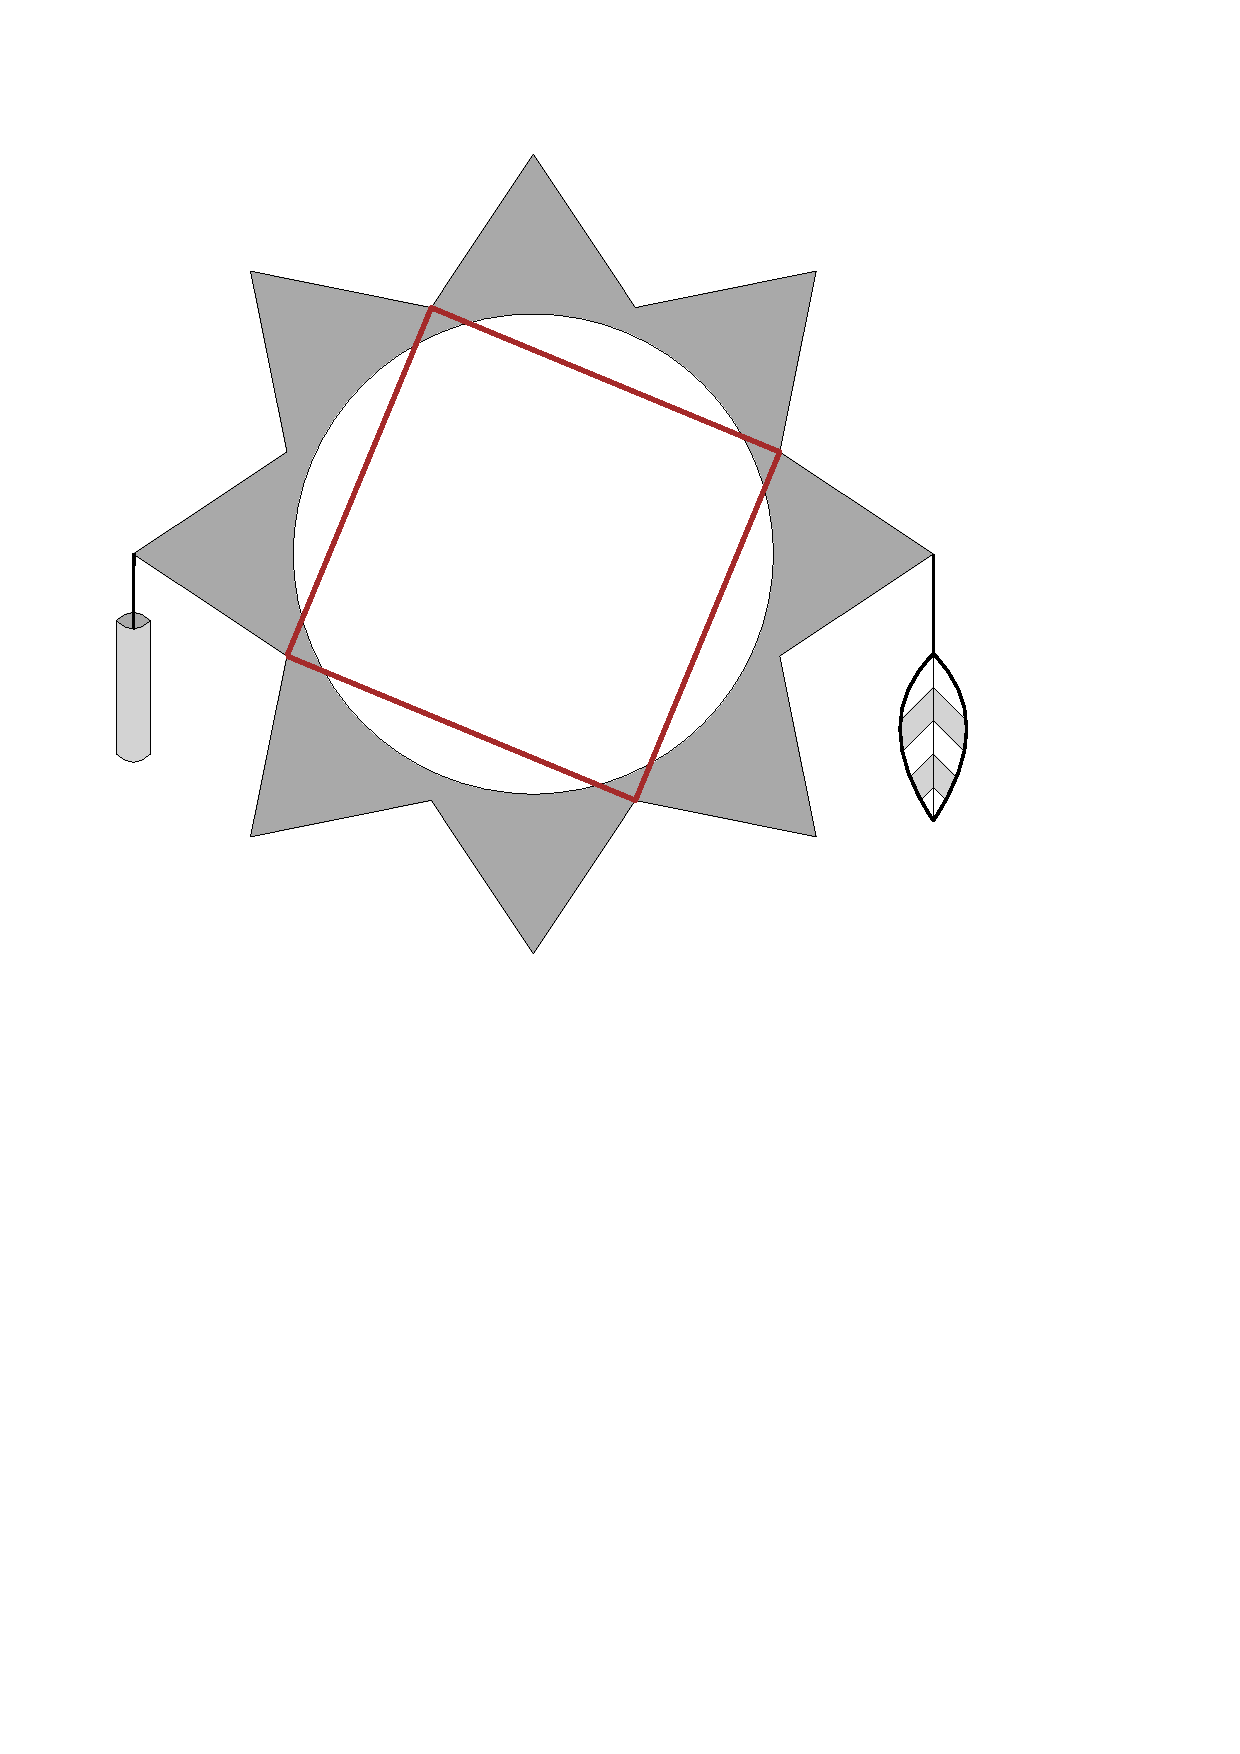
\includegraphics[width=3cm]{figure-n8-k2.pdf}
            \hfill
            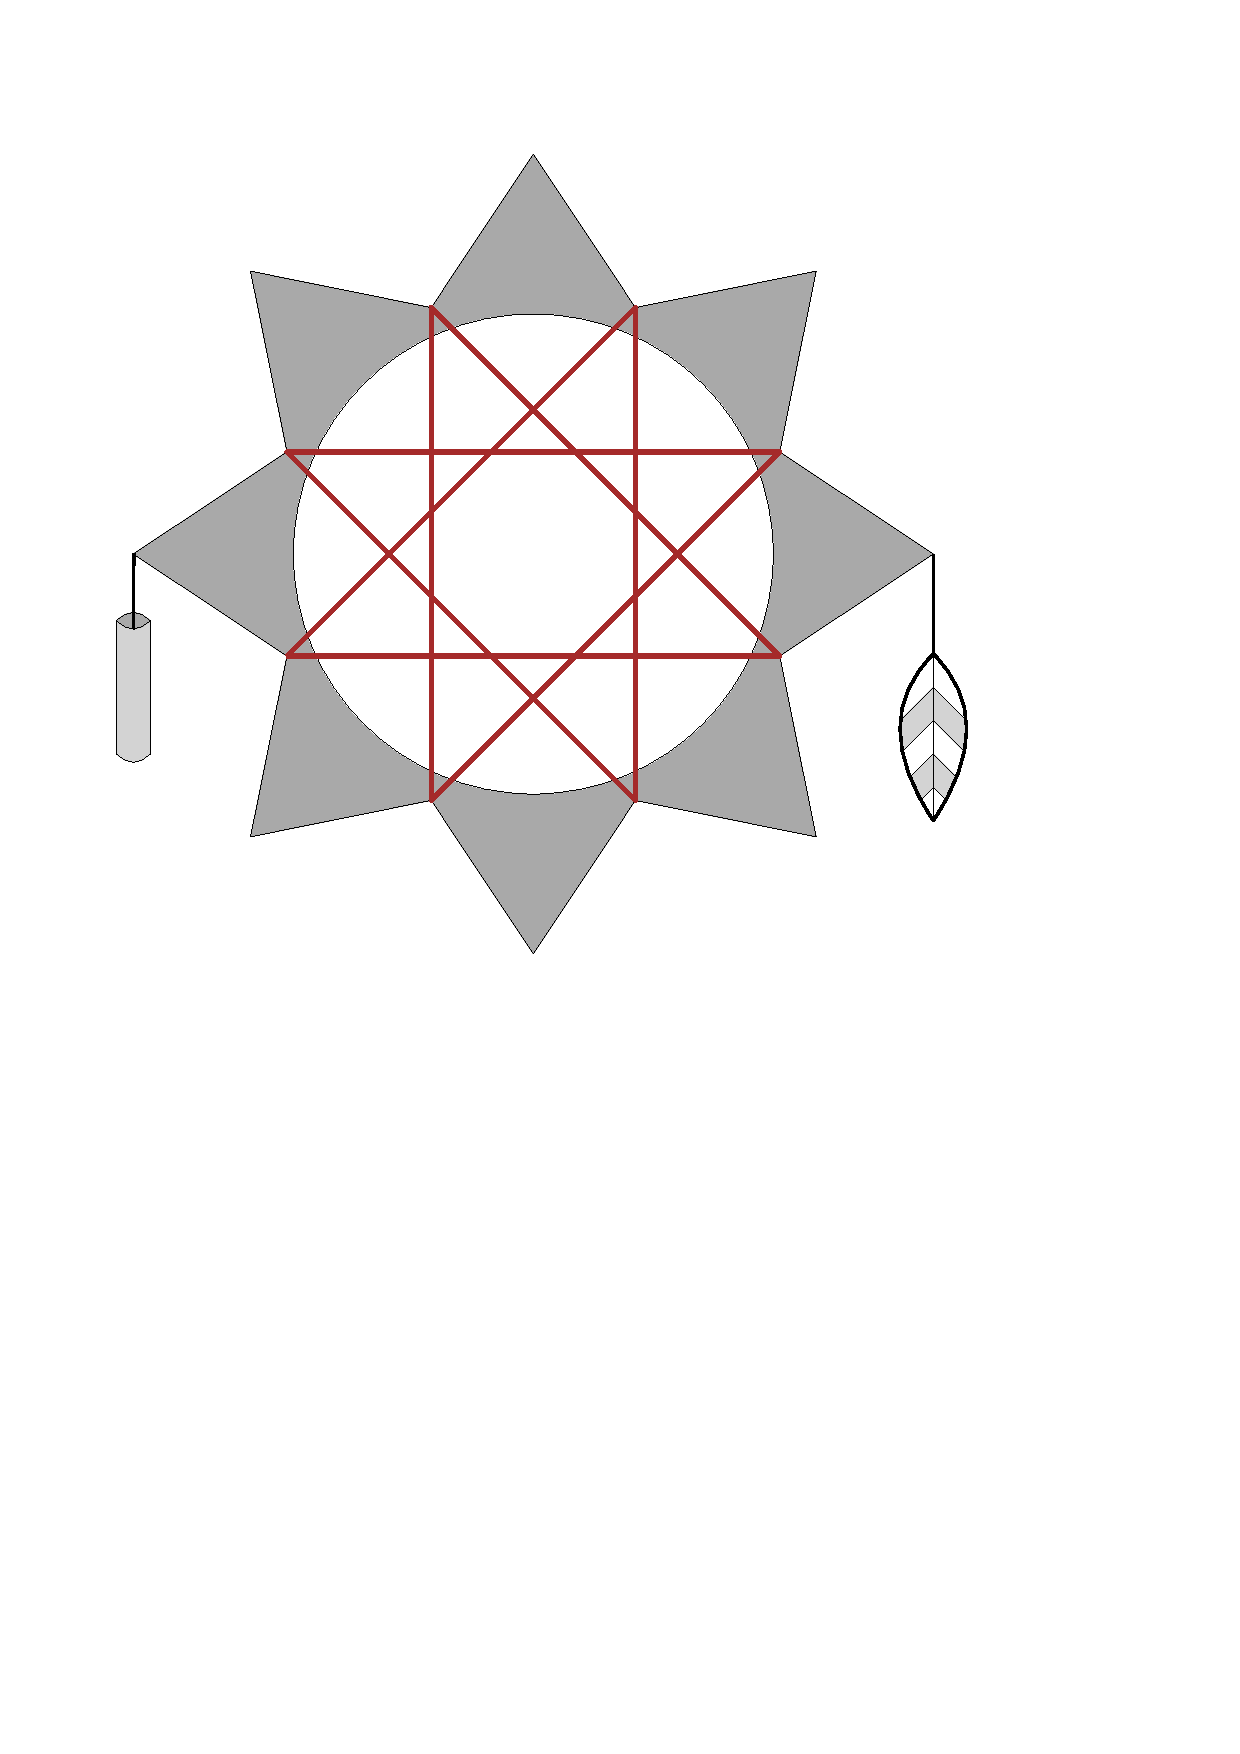
\includegraphics[width=3cm]{figure-n8-k3.pdf}
            \hfill
            \hfill% Silly LaTeX, requiring \hfill twice at the end of a line

            \small
            A dreamcatcher with $8$ notches, wrapped in a string of yarn for $k = 2$ and $k = 3$.
        \end{column}

        \illustration{0.25}{illustration.jpg}{
            Pixabay Content Licence by wal\_172619 on \href{https://pixabay.com/photos/dream-catcher-decoration-5731922/}{Pixabay}
        }
    \end{columns}
\end{frame}
